\section{Vorlesung 18.05.2016}

\subsection{Augenentwicklung bei Drosophila melanogaster}
\subsubsection{Festgelegte Reihenfolge der ommatidialen Zelldifferenzierung:}
\begin{enumerate}
	\item R8
	\item R2+R5
	\item R3+R4
	\item R1+R6
	\item R7
	\item Kristallkegelzelle
	\item primäre Pigmentzelle
	\item Sekundäre und tertiäre Pigmentzelle
\end{enumerate}
R8 = „Organisatorzelle“ (proneurales Potential durch atonal -Expression) laterale Inhibition der Nachbarzellen (sca) (nicht R8)\\

Differenzierung eines Zelltyps verändert die zelluläre Umwelt, wodurch neue Entwicklungsschritte angestoßen werden (induktive Wechselwirkung) $\Rightarrow$
Genetisch bedingte sukzessive Rekrutierung\\

\subsection{Morphogenetische Furche}
Inititation:\\
Dpp (Decapentaplegic\footnote{\url{https://en.wikipedia.org/wiki/Decapentaplegic}}) sezerniertes Molekül, Expression vor Aufreten der Furche am ventralen, dorsalen und posterioren Rand der Augenscheibe. Ektopische Expression von Dpp initiiert Furchenbildung andernorts.\\

Mutante: wingless. Exprimiert ein Dpp-Antagonist. Bei ausreichender Dpp-Überexpression kann wingless-Hemmung überwunden werden, aber es werden weitere Furchen (dorsal und ventral) gebildet\\

\subsubsection{Fortbewegung der Furche:}
hedgehog: Segmentpolaritätsgen, sezerniertes Molekül,\\
Expression direkt hinter der Furche\\
initiiert vor der Furche die Dpp-Expression\\
hedghogts-Allele: bei restriktiver Temperatur\\
kommt es zum Stillstand der Furche\\
(Vorteil ts-Allele !!)\\
roughex: Synchronisierung des Zellzyklus in der Furche durch Arretierung in der G1-Phase\\
Posterior der Furche gebildetes Hedehog induziert in den Zellen anterior der Furche die Expressionen von diversen Genen (z.B. ato). Durch Delta-Notch Signal verstärkt ato-Expression und innerhalb der Furche (während der Phase der lateralen Inhibition) erhält ato seine eigene Expression aufrecht. Diese ist jedoch sensibel gegenüber dem jetzt neurogenen Signal von sca/Notch, was schließlich die Reduktion der ato-Expression bewirkt.\\

Die Reichweite der lateralen Inhibition bestimmt die Anzahl und Muster der R8-Zellen.\\

\subsubsection{Sevenless – boss (\textbf{b}rides \textbf{o}f sevenle\textbf{ss}) Mutante}
Fehlen der Zelle R7 -$>$ diese werden als letzte Retinulazellen differenziert und detektieren UV-Licht.\\
Sevenless Genprodukt wird in zwei Polypedtidketten gespalten. Beide sind Membrangängig. Sevenless ist Rezeptor für Positionssignal, dass die R7-Vorläuferzelle zur R7 Zelle determiniert.\\

In Augenimaginalscheibe wird boss-Genprodukt nur in R8 gebildet. Heterophile Adhäsion zwischen boss- und sevenless-exprimierenden Zellen. Nur das Boss-Positionierungssignal enthält somit die Information über den richtigen Ort und den richtigen Zeitpunkt der R7-Entwicklung.\\

\subsection{Augenentwicklung: Vertebarten - Invetebraten}
Im Gegensatz zum Komplexauge der Insekten, welches aus einer Vielzahl von identischen Einzelaugen besteht, die jeweils aus wenigen Zellen aufgebaut sind, ist das Vertebratenauge ein einheitliches Organ von hoher Komplexität. Trotzdem spielen bei der Entwicklung viele der Gene eine Rolle, die bei der Entwicklung des Komplexauges der Insekten von Bedeutung sind. Insbesondere Start- und Endpunkt der Genkaskaden der Augenentwicklung sind in der Evolution konserviert. Bestes Beispiel eyeless / Pax-6 -$>$ Masterkontrollgene für Augenexpression.\\
Pax 6 (bei Maus): heterozygot: kleine Augen, homozygot: letal\\

Ein ganzes Bündel an Proteinen, vorgeschriebener Pfade und Signalkaskaden bilden ein kompliziertes regulatorisches Netzwerk und müssen zusammen funktionieren um das Komplexauge in Drosophila zu bilden.\\

\underline{Das C. Elegans Konnektom}
\begin{itemize}
	\item Einfaches Nervensystem
	\item 302 Neurone
	\item Zellschicksal und neurale Kreise vollständig dokumentiert
\end{itemize}

\underline{Konnektom:}
\begin{itemize}
	\item 302 Neurone
	\item 5000 chemische Synapsen
	\item 600 elektrische Synapsen
	\item 2000 Nerven-Muskel Synapsen
\end{itemize}

\underline{Neuronen können unterteilt werden in:}
\begin{itemize}
	\item Interneuronen
	\item Sensorische Neuronen
	\item Motorneuronen
\end{itemize}

\underline{Kopfneurone:}
\begin{itemize}
	\item Der Nervenring enthält überwiegend sensorische Neurone und fast alle Interneurons
	\item Der Nervenring ist das Gehirn von C. Elegans
\end{itemize}

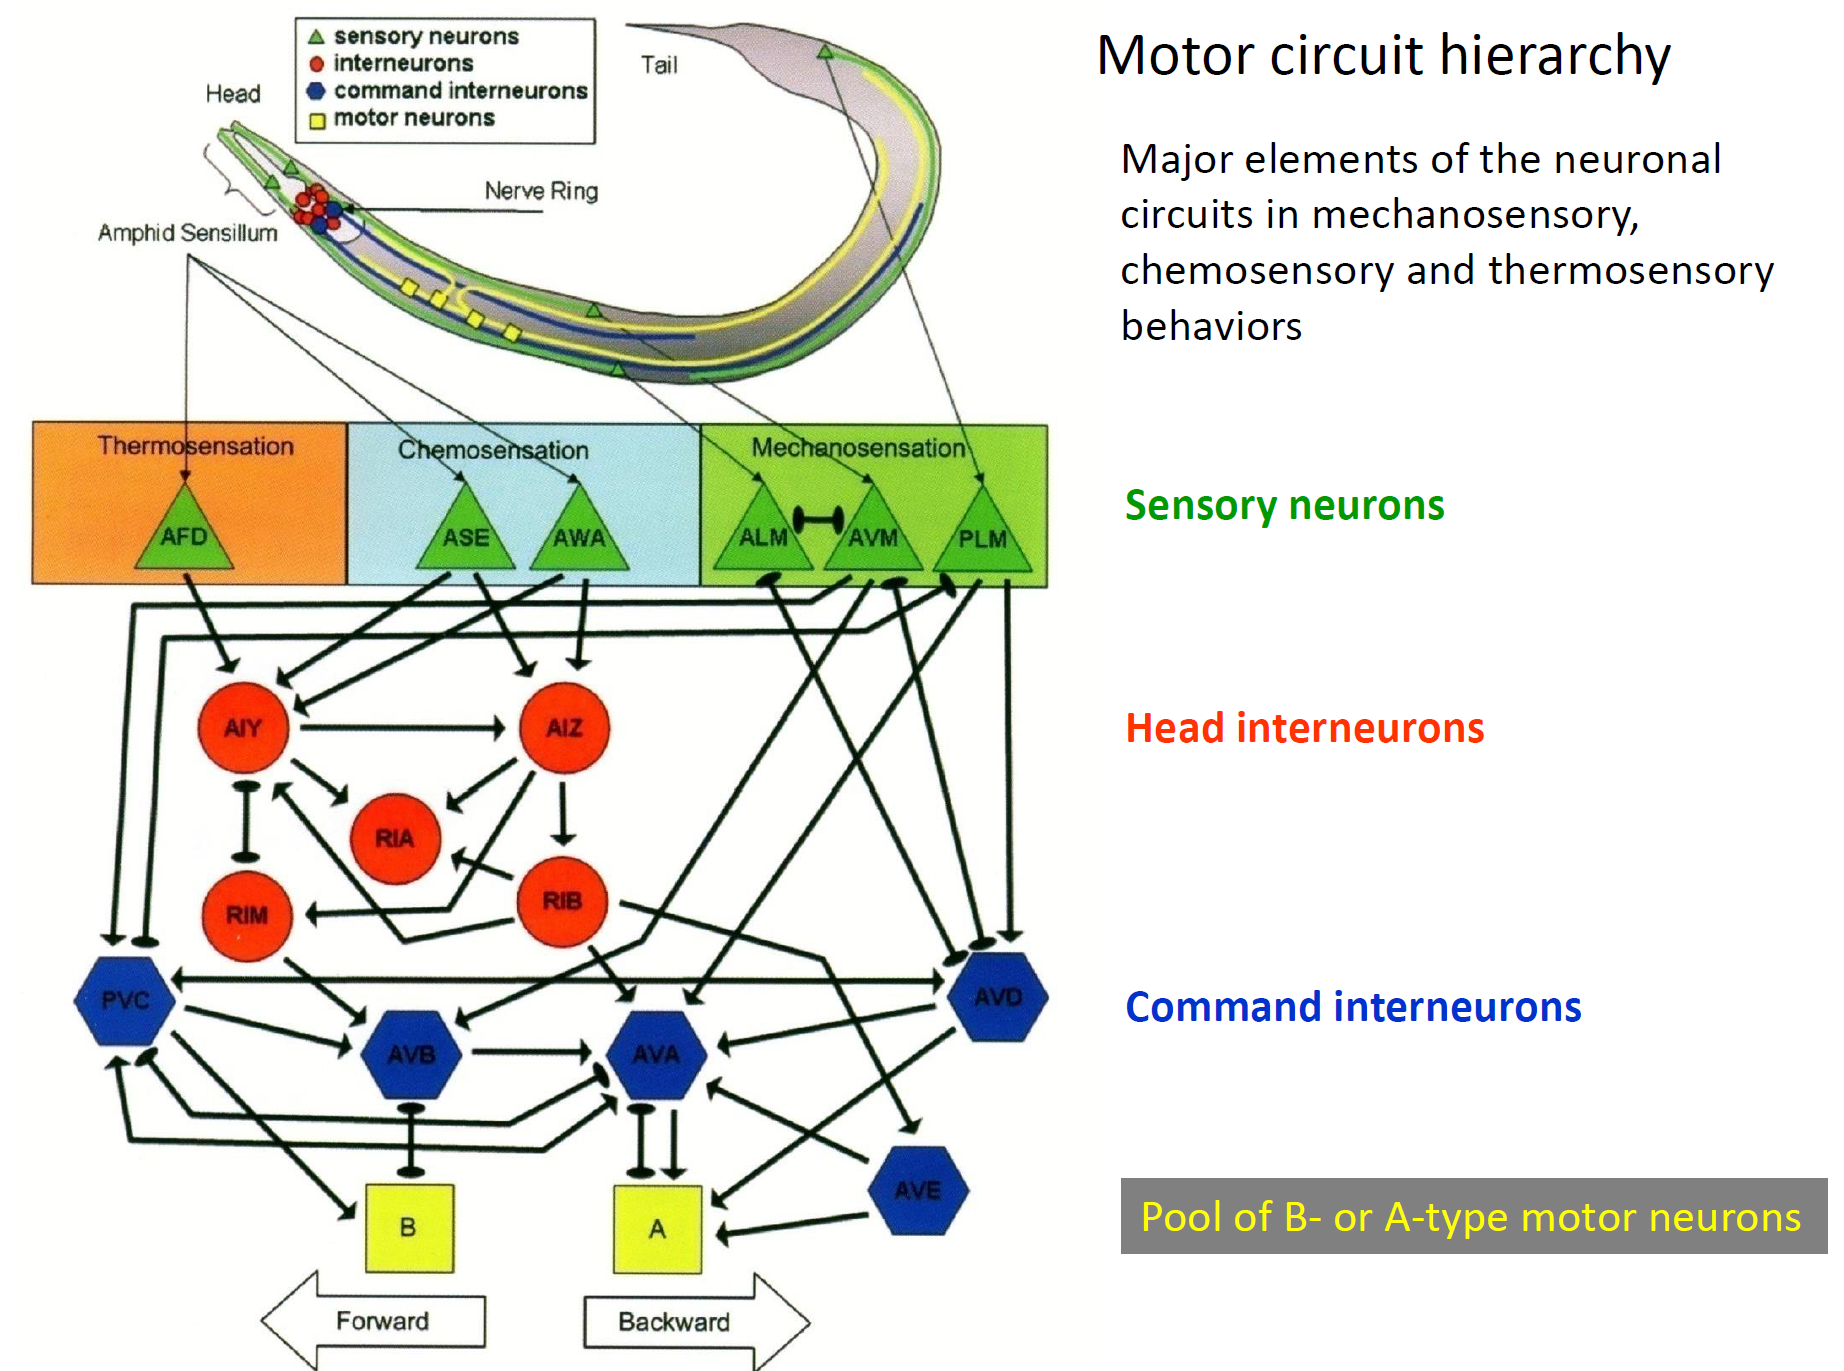
\includegraphics[width=1\textwidth]{lectures/160511/pix/c_elegans_neurones.png}
\\\\
Netzwerk von C. Elegans ist überschaubar. Aber wir wird es gebildet und wie kann man Zugriff darauf erlangen.\\


\subsection{Struktur -- Funktion: Axonale Wegfindung in der Entwicklung}
\underline{Beispiel irreC [irregular chiasma] Mutante von Drosophila)}
Retinotrope Projektion im Wachstum: Aufrechterhaltung von Nachbarschaftsbeziehungen aus den Augen in den Loben (d.h.: richtige Säule und richtige Schicht)\\

IrreC-Mutation: Fehlerhaftes axonales Wachstum bei R7-, R8-, Laminarmonopolarzellaxonen\\

Struktur-Funktion: Axonales Wachstum, Zellwanderung
\begin{enumerate}
	\item Axonales Wachstum
	\item Zielerkennung
	\item Ausbildung spezifischer Kontakte
\end{enumerate}

Insbesondere bei Vertebraten: Wanderung undifferenzierter Neurone.
Regulative Mechanismen in beiden Fällen ähnlich. Abhängig von Signal-Erkennungs-Mechanismen, nicht zellautonom.\\

Beispiel: Zellen des peripheren Nervensystems (PNS) entstehen in der Neuralleiste und wandern aus, um Ganglien des PNS zu bilden.